\documentclass[thesis.tex]{subfiles}

\begin{document}
\chapter{Performance testing}
\label{sec:performance}
This chapter is concerned with testing the efficiency of the approach by running large scale tests on the implemented tool. There are two metrics which will be presented: The running time of the algorithm and the correctness of the achieved result. How correctness is determined is covered in section \ref{sec:performance_validation}. Most of the results are compared against running the same alignment with an own PO-MSA implementation. We chose PO-MSA because of its intuitive nature, the easily deducible relationship between graph complexity and running time and, most importantly, because it is a non-heuristical approach guaranteeing a correct result every time.
\section{Test data}
These tests are meant to reflect usage in a what would be an every day situation, and does therefore use real genetic data. All of the sequences are FASTA-files from the MHC region fetched from the vg github repo\cite{vg} and the test-set provided by the sequence graphs tool\cite{sequence_graphs}. The exact test sets are chosen to provide a variety of sequence lengths. In order to cover lengths where we found no sequences there are created artificial sequences by cutting out suitable regions from longer sequences. All the sequences which are used can be found in the test-folder of the github repo of the tool.\\
\par\noindent
Specifically, there are 8 main data-sets involved in the testing process:
\begin{itemize}
  \item \textbf{mhc1.fa} A 700 bp long sequence from the MHC region (not specified more precisely where). Fetched from the docker repo of the sg project
  \item \textbf{primary.fasta} A 3345 bp long sequence from the HLA-A gene in the MHC region from the primary assembly of GRCh38. Originates from the vg github.
  \item \textbf{20k.fasta, 35k.fasta, 100k.fasta, 150k.fasta, 500k.fasta} Five subsequences of an alternate assembly of the MHC region of respectively 21.070bp, 35.770bp, 101.570bp, 144.480bp and 448.490bp. The alternate assembly originates from the NCBI database\cite{ncbi} with id NT\_167244.1.
  \item \textbf{mhc\_full.fa} The previously mentioned full mhc assembly of 4.622.290bp.
\end{itemize}
Additionally, some of the tests use more specific data, to test specific properties. This data will be presented before it is used.\\
\par\noindent
In order to do alignments we need reads aswell as the data used in building the reference structure. These reads are generated by the read-generator seen in the appendix. A read $r$ from a graph $G$ is generated by the following procedure:
\begin{enumerate}
  \item Choose a random vertex $v \in V\setminus\{s_G, t_G\}$ such that the smallest distance from $v$ to $t_g$ is larger than the chosen read size $|r|$
  \item For $|r|$ steps:
  \begin{enumerate}
    \item Append $b(v_x)$ to the read $r$
    \item Choose a random neighbouring vertex $v_y \in n_o(v_x)$ as the new $v_x$
  \end{enumerate}
  \item When a read $r$ has been generated, for $r_i \in r$
  \begin{enumerate}
    \item Choose a random floating point value $0<=v<=1$
    \begin{itemize}
      \item If $v<(p/3)$ delete $r_i$
      \item Else if $v<(2p/3)$ insert a random base $b \in \{A, C, G, T\}$ before $r_i$
      \item Else if $v<p$ substitue $r_i$ with a random base $b \in \{A, C, G, T\}\setminus\{r_i\}$
    \end{itemize}
  \end{enumerate}
  \item Output $r$
\end{enumerate}
In order to provide reproducability the randomness in the reads are generated from a seed.\\
\par\noindent
Because this thesis is concerned with the mathematical properties of the model the noise in the reads does not necessarily depict the true nature of either genetic variation (Section \ref{sec:genetic_variation}) or read errors (Section \ref{sec:sequencing}). This is one of the points where we have chosen to limit the complexity of the problem. \textcolor{red}{As long as we see the approach as a solution to the most general problem we argue this is an acceptable limitation.}
\section{Validation}
\label{sec:performance_validation}
When an alignment is produced for a read we classify it as either as correct or not correct. Intuitively one could imagine this can be figured out by determining whether the generated read aligns back to the path it was generated from. However, when noise is introduced an interesting phenomenon can occur: The modified read can become more similar to another path in the graph than its origin. This can also occur whenever there exists actual equal paths in the graph, typically in the case of repeats. In order to stick with mathemathical properties, our definition of optimality holds no relation to the origin of a read but is purely defined as the path which produces the highest possible alignment score. As PO-MSA is an exhaustive search we define optimally aligned as alignments which produce the same alignment score as the highest score found by PO-MSA. Consequently, as only the scores are compared, even when the approach produces a different alignment than PO-MSA, this is classified as optimal behaviour. Correctness is only discussed in the later stages of the chapter. This is because of the non-heuristical properties of the algorithm: We are able to devise parameters and test data in such a way that correctness is not an interesting measurement. In all tests where accuracy is omitted this is because the approach had a 100\% success rate.
\par\noindent
\section{Time capturing mechanisms}
For both the "Fuzzy context-based search" and the PO-MSA algorithm the time capturing mechanisms are built into the tool, using the Java System object. This allows us to wrap the time capturing of each individual constituent as close to the functional parts as possible in order to avoid unecessary overhead. When comparing tools the time was taken from the tool was started until the tool ended. Doing it this way has several disadvantages, which are discussed in Section \ref{sec:comparison_tools}. The time unit used throughout the chapter is milliseconds.
\section{Building the index}
The building of the index is the first step of the process realized through the build\_index.sh script. To summarize this step consists of reading the input files, building the graph and generating the suffix trees. The build process was run 50 times on 6 different data sets, the averaged results can be seen in figure \ref{fig:build_index}. All of these are linear operations, a trend which is clearly visible. The tool was not able to build an index for the largest input file with ~4.5mb because of insufficient memory.\\

\begin{figure}[!ht]
    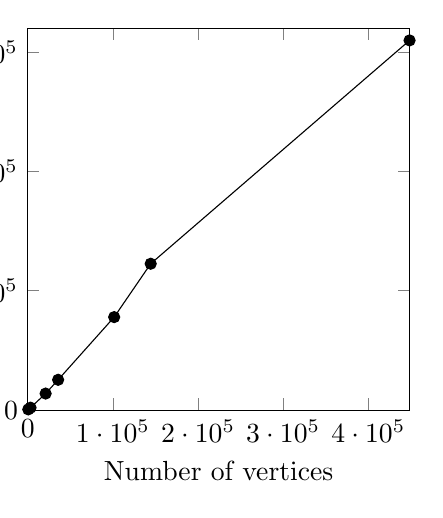
\begin{tikzpicture}[trim axis left, trim axis left]
      \begin{axis}[scale only axis,height=0.4\textwidth,width=0.4\textwidth,xmin=0,ymin=0,xmax=448490,ymax=320000,scaled ticks=false, xlabel={Number of vertices}, ylabel={Milliseconds}, max space between ticks=50pt, ylabel near ticks]
        \addplot[color=black,mark=*] coordinates {
          (700,597)
          (3345,2050)
          (21070,13858)
          (35770,25401)
          (101570,77928)
          (144480,122654)
          (448490,309791)
        };
      \end{axis}
    \end{tikzpicture}
    \caption{Runtime for the build index procedure}
    \label{fig:build_index}
\end{figure}
\par\noindent
When splitting up the runtime into the individual constituents an interesting pattern emerges: The main load of the indexation lies in writing to file (Figure \ref{fig:index_constituents}). The data structure used is a large tree of nested complex structures, which the standard Java serialization does not handle well \textcolor{red}{PROB SHUD REFERENCE SOMETHING. API MAYBE}. Putting effort into improved serialization or reducing the size of the index will thus have a dramatic effect on the time complexity.
\begin{figure}[!t]
  \begin{subfigure}[t]{0.4\textwidth}
    \begin{tikzpicture}[trim axis left]
      \begin{axis}[scale only axis,height=\textwidth,width=\textwidth,xmin=0,ymin=0,xmax=144480,ymax=320000,scaled ticks=false]
        \addplot coordinates {
          (700,9)
          (3345,51)
          (21070,623)
          (35770,1031)
          (101570,5487)
          (144480,11328)
        };
      \end{axis}
    \end{tikzpicture}
    \subcaption{Time used building the graph}
  \end{subfigure}
  \hfill
  \begin{subfigure}[t]{0.4\textwidth}
    \begin{tikzpicture}[trim axis left]
      \begin{axis}[scale only axis,height=\textwidth,width=\textwidth,xmin=0,ymin=0,xmax=144480,ymax=125000,scaled ticks=false]
        \addplot[color=green,mark=*] coordinates {
          (701,65)
          (3345,138)
          (21070,269)
          (35770,2788)
          (101570,6905)
          (144480,10007)
        };
      \end{axis}
    \end{tikzpicture}
    \subcaption{Time used building the index}
  \end{subfigure}
  \begin{subfigure}[b]{0.4\textwidth}
    \begin{tikzpicture}[trim axis left]
      \begin{axis}[scale only axis,height=\textwidth,width=\textwidth,xmin=0,ymin=0,xmax=144480,ymax=125000,scaled ticks=false]
        \addplot[color=red,mark=*] coordinates {
          (700,522)
          (3345,1860)
          (21070,12960)
          (35770,21581)
          (101570,65535)
          (144480,101317)
        };
      \end{axis}
    \end{tikzpicture}
    \subcaption{Time used writing the index\vspace{\baselineskip}}
  \end{subfigure}
  \hfill
  \begin{subfigure}[b]{0.4\textwidth}
  \begin{tikzpicture}[trim axis left]
    \begin{axis}[scale only axis,height=\textwidth,width=\textwidth,xmin=0,ymin=0,xmax=144480,ymax=125000,scaled ticks=false]
      \addplot[color=blue,name path=graph] coordinates {
        (700,9)
        (3345,51)
        (21070,623)
        (35770,1031)
        (101570,5487)
        (144480,11328)
      };
      \addplot[color=green, name path=index] coordinates {
        (700,9 + 65)
        (3345,51 + 138)
        (21070,623 + 269)
        (35770,1031 + 2788)
        (101570,5487 + 6905)
        (144480,11328 + 10007)
      };
      \addplot[color=black, name path=total,mark=*] coordinates {
        (700,597)
        (3345,2050)
        (21070,13858)
        (35770,25401)
        (101570,77928)
        (144480,122654)
      };
      \addplot[name path=axis] coordinates {
        (0, 0)
        (144480, 0)
      };
      \addplot[red!30] fill between[of=index and total];
      \addplot[green!30] fill between[of=graph and index];
      \addplot[blue!30] fill between[of=graph and axis];
      \addlegendentry{Build graph}
      \addlegendentry{Build index}
      \addlegendentry{Write index}
    \end{axis}
  \end{tikzpicture}
  \subcaption{Total run time as a combination of the individual steps}
  \label{fig:index_constituents_explicit}
  \end{subfigure}
  \caption{Time used by the individual constituents of the build index process}
  \label{fig:index_constituents}
\end{figure}
\clearpage
\section{Alignment}
The alignment tests are run by the align\_sequence.sh script, both with \texttt{-{}-type=fuzzy} and \texttt{-{}-type=po\_msa} parameters. The section is divided into segments, based on what variable is tuned. As a remainder to the reader, these are the variables which are in play:
\begin{itemize}
  \item $|G|$ is the size of the graph
  \item $\lambda$ is the allowed error margin
  \item $|s|$ is the length of the input sequence
  \item $b$ is the branching factor of the graph
\end{itemize}
Additionally we include one more variable:
\begin{itemize}
  \item $p$ is the amount of noise added to the reads
\end{itemize}
As each of the subsequent sections are concerned with the impact of exactly one of these variables, the ``non-important'' variables are locked to a standard value:
\begin{itemize}
  \item $\mathbf{|G|=35.000}$ Representing the mid-range of our test-sets.
  \item $\lambda\mathbf{=0, p=0.0}$ We let alignment back to the origin represent the base case in the study.
  \item $\mathbf{|s|=120}$ Common read length for the Illumina HiSeq3000/4000 technology.
  \item $\mathbf{b=1}$ Calculations can be found in section \ref{sec:runtime_complexity} which is concerned with tuning this variable.
\end{itemize}
\subsection*{Runtime as a function of graph size}
We start by comparing the two alignment algorithms on different graph sizes. Figure \ref{fig:runtime_G} shows the averaged results over 50 runs of each algorithm on the smallest 6 datasets. The two largest datasets were omitted to avoid blowing the scale. As expected PO-MSA is completely linear with regards to the number of vertices. The fuzzy search is only dependant on the graph size to decide the depth of the suffix tree which needs to be searched in the first step, and the extremely logarithmical relationship comes across almost as constant in comparison.
\clearpage
\begin{figure}[!ht]
  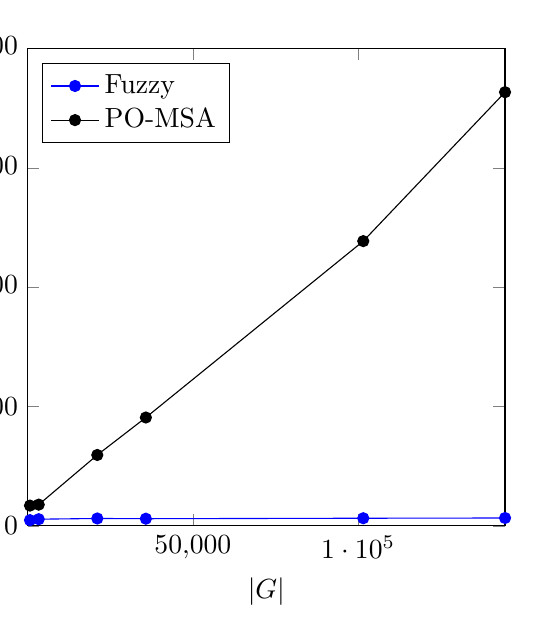
\begin{tikzpicture}[trim axis left, trim axis right]
    \begin{axis}[scale only axis,height=0.5\textwidth,width=0.5\textwidth,xmin=0,ymin=0,xmax=144480,ymax=2000,scaled ticks=false, legend pos=north west, xlabel={$|G|$}, ylabel={Milliseconds}, legend cell align=left, xtick={50000,100000,150000},ylabel near ticks]
      \addplot[color=blue,mark=*] coordinates {
        (700, 24)
        (3345, 28)
        (21070, 31)
        (35770,  30)
        (101570, 32)
        (144480, 33)
      };
      \addplot[color=black,mark=*] coordinates {
        (700, 85)
        (3345, 89)
        (21070, 297)
        (35770, 454)
        (101570, 1193)
        (144480, 1817)
      };
      \addlegendentry{Fuzzy}
      \addlegendentry{PO-MSA}
    \end{axis}
  \end{tikzpicture}
  \caption{Runtime of the alignment process as a function of $|G|$}
  \label{fig:runtime_G}
\end{figure}
\subsection*{Runtime as a function of error margin}
We vary the error margin by giving the algorithm different $\lambda$-values through the \texttt{-{}-error-margin} parameter. The results from 50 runs at 5 different values are seen in figure \ref{fig:runtime_lambda}. We can see an exponential growth, which is expected from the complexity analysis\footnote{Found in Appendix \ref{sec:complexity_analysis}}. Disconcertingly, the algorithm quickly overtakes PO-MSA, already at $\lambda=2$ the straight forward search is more efficient. Utilizing the results from the previous experiment we can identify that the starting point of the exponential growth is dependant on the graph size. Figure \ref{fig:runtime_lambda_parallell} shows the same set of tests on the larger graph, where we can see that the approach is more efficient up to $\lambda=2$. In the same figure we can see that the naive parallellization can soften the exponential growth by a linear factor, at the cost of an initial overhead.\\
\par\noindent
It is important to point out that the extreme growth in relation to the small numbers is in part determined by the flat scoring system. The exponential growth is related to the number of possibilities given $\lambda$, not necessarily $\lambda$ itself. A more fine grained scoring schema might produce a less explosive growth.\\
\begin{figure}[!hb]
  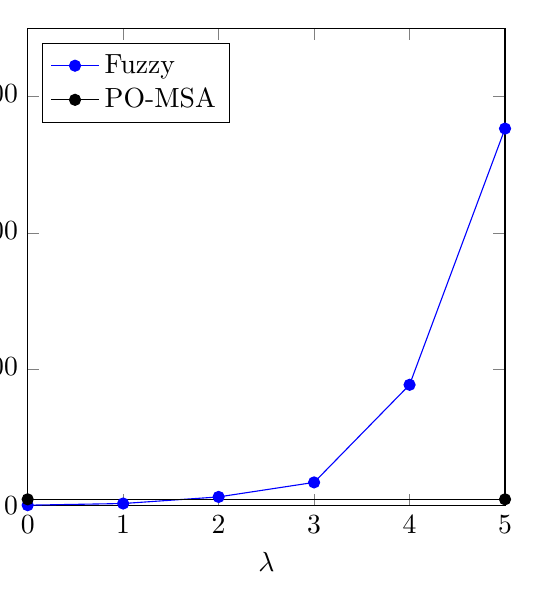
\begin{tikzpicture}[trim axis left, trim axis right]
    \begin{axis}[scale only axis,height=0.5\textwidth,width=0.5\textwidth,xmin=0,ymin=0,xmax=5,ymax=35000,scaled ticks=false, legend pos=north west, xlabel={$\lambda$}, ylabel={Milliseconds},xtick={0,1,2,3,4,5}, legend cell align=left, ylabel near ticks]
      \addplot[color=blue,mark=*] coordinates {
        (0, 29)
        (1, 152)
        (2, 636)
        (3, 1700)
        (4, 8856)
        (5, 27642)
      };
      \addplot[color=black,mark=*] coordinates {
        (0, 460)
        (5, 460)
      };
      \addlegendentry{Fuzzy}
      \addlegendentry{PO-MSA}
    \end{axis}
  \end{tikzpicture}
  \caption{Runtime of the alignment process as a function of $\lambda$}
  \label{fig:runtime_lambda}
\end{figure}
\begin{figure}
  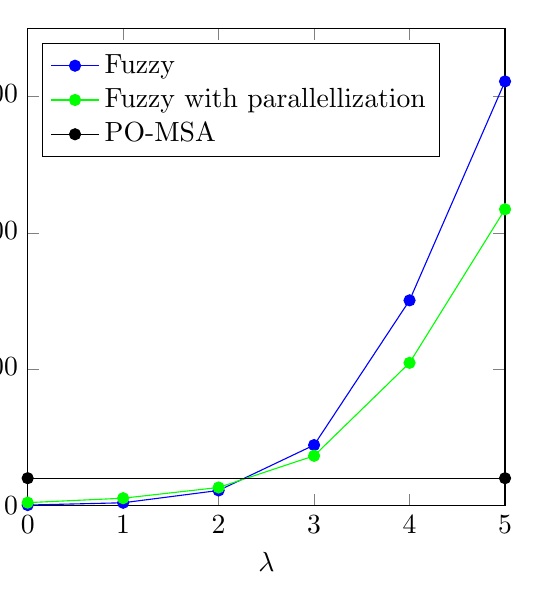
\begin{tikzpicture}[trim axis left, trim axis right]
    \begin{axis}[scale only axis,height=0.5\textwidth,width=0.5\textwidth,xmin=0,ymin=0,xmax=5,ymax=35000,scaled ticks=false, legend pos=north west, xlabel={$\lambda$}, ylabel={Milliseconds},xtick={0,1,2,3,4,5}, legend cell align=left, ylabel near ticks]
      \addplot[color=blue,mark=*] coordinates {
        (0, 39)
        (1, 207)
        (2, 1109)
        (3, 4438)
        (4, 15048)
        (5, 31101)
      };
      \addplot[color=green,mark=*] coordinates {
        (0,217)
        (1,541)
        (2,1327)
        (3,3649)
        (4,10466)
        (5,21725)
      };
      \addplot[color=black,mark=*] coordinates {
        (0, 2008)
        (5, 2008)
      };
      \addlegendentry{Fuzzy}
      \addlegendentry{Fuzzy with parallellization}
      \addlegendentry{PO-MSA}
    \end{axis}
  \end{tikzpicture}
  \caption[Runtime of the alignment process as a function of $\lambda$ with a larger data set]{Runtime of the alignment process as a function of $\lambda$ with $|G|=150.000$ and \texttt{-{}-parallellization=true}}
  \label{fig:runtime_lambda_parallell}
\end{figure}
\clearpage
\subsection*{Runtime as a function of sequence length}
We vary the sequence lengths through changing the lengths produced by the read generator. The read lengths are taken from a set of sequencing machines, chosen to portray a diversity of read lengths\textcolor{red}{ref}. Both the technologies, the lengths and the runtimes are listed in table \ref{tab:runtimes_s}. The number are visualized in figure \ref{fig:runtime_s}
\begin{table}[!h]
  \begin{tabular}{|l|l|r|r|}
    \hline \textbf{Technology} & \textbf{Read length} & \textbf{PO-MSA time} & \textbf{Fuzzy time} \\ \hline
    HiSeq2000 (min) & 50 & 171 & 19 \\ \hline
    SOLiDv4 & 100 & 294 & 36 \\ \hline
    HiSeq3000/4000 & 120 & 0 & 0 \\ \hline
    Ion PGM & 200 & 676 & 59 \\ \hline
    Sanger 3730xl (min) & 400 & 1117 & 98 \\ \hline
    454 GS FLX & 700 & 1600 & 167 \\ \hline
    Sanger 3730xl (max) & 900 & 2121 & 194 \\ \hline
  \end{tabular}
  \caption{Running times for different read lengths for the PO-MSA and fuzzy algorithms}
  \label{tab:runtimes_s}
\end{table}
\begin{figure}[!hb]
  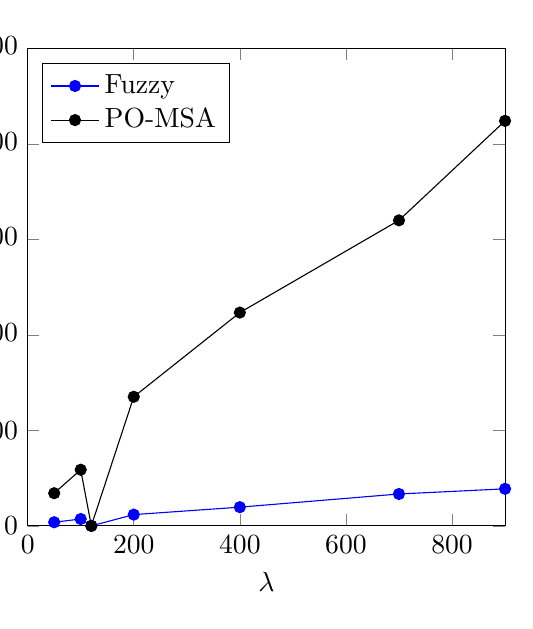
\begin{tikzpicture}[trim axis left, trim axis right]
    \begin{axis}[scale only axis,height=0.5\textwidth,width=0.5\textwidth,xmin=0,ymin=0,xmax=900,ymax=2500,scaled ticks=false, legend pos=north west, xlabel={$\lambda$}, ylabel={Milliseconds}, legend cell align=left, ylabel near ticks]
      \addplot[color=blue,mark=*] coordinates {
        (50,19)
        (100,36)
        (120,0)
        (200,59)
        (400,98)
        (700,167)
        (900,194)
      };
      \addplot[color=black,mark=*] coordinates {
        (50,171)
        (100,294)
        (120,0)
        (200,676)
        (400,1117)
        (700,1600)
        (900,2121)
      };
      \addlegendentry{Fuzzy}
      \addlegendentry{PO-MSA}
    \end{axis}
  \end{tikzpicture}
  \caption{Runtime of the alignment process as a function of $|s|$}
  \label{fig:runtime_s}
\end{figure}
\clearpage
\subsection*{Runtime as a function of graph complexity}
\label{sec:runtime_complexity}
We let the branching probability $b$ denote the complexity of our graph. We generated vcf-files with the read-generator to provide a variety of values. The results of running alignments against each of the indexes can be seen in figure \ref{fig:runtime_b}. As seen in the table, the experiment was run on rather moderate values. If we use the numbers from section \ref{sec:human_genome}, assuming all variants are singular and specific to a single individual, a population graph of the human genome would have a branching factor $b=1+|p|*0000076$, where $|p|$ denotes the number of individuals\footnote{23.000 variants/3.000.000.000bp}. In this case the largest branching factor presented in the figure would cover a a population of 10.000. In the far more probable case of overlapping and complex variants the number will be larger. \textcolor{red}{Needs more tests and more motivation behind the sizes}. It is important to remember the number of variants present in the graph is an exponential combination of both $b$ and the graph size.
\begin{figure}[!hb]
  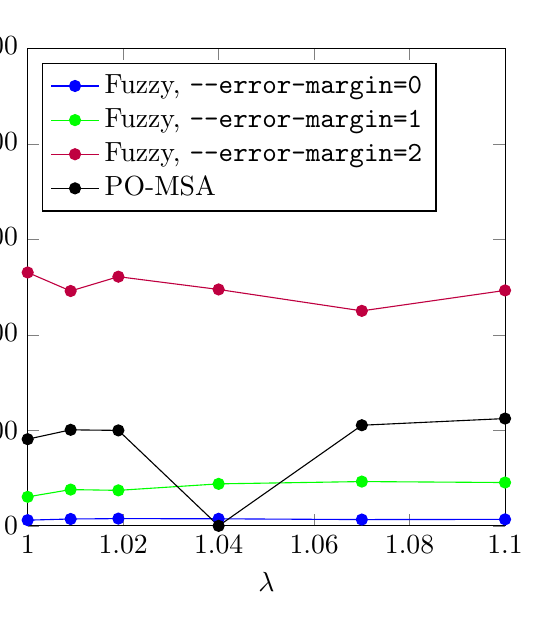
\begin{tikzpicture}[trim axis left, trim axis right]
    \begin{axis}[scale only axis,height=0.5\textwidth,width=0.5\textwidth,xmin=1,ymin=0,xmax=900,ymax=2500,xmax=1.1,scaled ticks=false, legend pos=north west, xlabel={$\lambda$}, ylabel={Milliseconds}, legend cell align=left, ylabel near ticks]
      \addplot[color=blue,mark=*] coordinates {
        (1,30)
        (1.009,36)
        (1.019,38)
        (1.04,37)
        (1.07,33)
        (1.1,34)
      };
      \addplot[color=green,mark=*] coordinates {
        (1,152)
        (1.009,190)
        (1.019,186)
        (1.04,220)
        (1.07,232)
        (1.1,227)
      };
      \addplot[color=purple,mark=*] coordinates {
        (1,1327)
        (1.009,1230)
        (1.019,1305)
        (1.04,1238)
        (1.07,1126)
        (1.1,1233)
      };
      \addplot[color=black,mark=*] coordinates {
        (1,454)
        (1.009,503)
        (1.019,500)
        (1.04,0)
        (1.07,527)
        (1.1,562)
      };
      \addlegendentry{Fuzzy, \texttt{-{}-error-margin=0}}
      \addlegendentry{Fuzzy, \texttt{-{}-error-margin=1}}
      \addlegendentry{Fuzzy, \texttt{-{}-error-margin=2}}
      \addlegendentry{PO-MSA}
    \end{axis}
  \end{tikzpicture}
  \caption{Runtime of the alignment process as a function of $b$}
  \label{fig:runtime_b}
\end{figure}
\clearpage
\subsection*{Correctness as a function of noise}
In the previous tests we have guaranteed correct results through the tuning of input parameters. We will now introduce a level of uncertainty through introducing randomness to our reads through the noise parameter $p$. To some degree this is a futile exercise: We will get correct results when the number of modifications is lower then $\lambda$ and empty alignments in the remaining cases, mirroring the distribution of the underlying randomness. This is however interesting as a depiction of a real life situation where the noise is to some degree uncertain. The percentage of correctly aligned reads over 100 runs with a variety of settings is seen in figure \ref{fig:correctness}. The regular algorithm, seen in \ref{fig:correctness_both}, shows a clear linear relationship between $p$ and $\lambda$. This will be the first set of tests where we also include the results from the heuristical algorithm, shown in \ref{fig:correctness_both_heur}
\begin{figure}[!hb]
  \begin{subfigure}[t]{0.49\textwidth}
  \begin{center}
    \begin{tikzpicture}[every node/.style={anchor=base,text depth=.5ex,text height=1.55em,text width=1.55em},align=center,text centered, trim axis left, trim axis right]
      \matrix(A) [nodes={rectangle}] {
        \node {5}; & \HeatmapNode{100} & \HeatmapNode{100} & \HeatmapNode{99} & \HeatmapNode{96} & \HeatmapNode{83} & \HeatmapNode{80}\\
        \node {4}; & \HeatmapNode{100} & \HeatmapNode{99} & \HeatmapNode{96} & \HeatmapNode{83} & \HeatmapNode{73} & \HeatmapNode{61}\\
        \node {3}; & \HeatmapNode{100} & \HeatmapNode{97} & \HeatmapNode{87} & \HeatmapNode{76} & \HeatmapNode{52} & \HeatmapNode{45}\\
        \node {2}; & \HeatmapNode{100} & \HeatmapNode{93} & \HeatmapNode{73} & \HeatmapNode{59} & \HeatmapNode{44} & \HeatmapNode{41}\\
        \node {1}; & \HeatmapNode{100} & \HeatmapNode{84} & \HeatmapNode{55} & \HeatmapNode{38} & \HeatmapNode{36} & \HeatmapNode{25}\\
        \node {0}; & \HeatmapNode{100} & \HeatmapNode{79} & \HeatmapNode{38} & \HeatmapNode{18} & \HeatmapNode{10} & \HeatmapNode{4}\\
        \node {};  & \node{0}; & \node{0.01}; & \node{0.02}; & \node{0.03}; & \node{0.04}; & \node{0.05}; \\
      };
      \node[draw=none] at (0.5, -0.75) {$p$};
      \node[draw=none] at (-3, 3.25) {$\lambda$};
    \end{tikzpicture}
  \end{center}
  \subcaption{\texttt{-{}-heuristical=false}}
  \label{fig:correctness_both}

  \hfill
  \end{subfigure}
    \begin{subfigure}[t]{0.49\textwidth}
  \begin{center}
    \begin{tikzpicture}[every node/.style={anchor=base,text depth=.5ex,text height=1.55em,text width=1.55em},align=center,text centered, trim axis left, trim axis right]
      \matrix(A) [nodes={rectangle}] {
        \node {5}; & \HeatmapNode{100} & \HeatmapNode{100} & \HeatmapNode{100} & \HeatmapNode{98} & \HeatmapNode{100} & \HeatmapNode{100}\\
        \node {4}; & \HeatmapNode{100} & \HeatmapNode{100} & \HeatmapNode{100} & \HeatmapNode{100} & \HeatmapNode{97} & \HeatmapNode{98}\\
        \node {3}; & \HeatmapNode{100} & \HeatmapNode{99} & \HeatmapNode{100} & \HeatmapNode{94} & \HeatmapNode{83} & \HeatmapNode{79}\\
        \node {2}; & \HeatmapNode{100} & \HeatmapNode{97} & \HeatmapNode{97} & \HeatmapNode{91} & \HeatmapNode{79} & \HeatmapNode{69}\\
        \node {1}; & \HeatmapNode{100} & \HeatmapNode{91} & \HeatmapNode{75} & \HeatmapNode{51} & \HeatmapNode{46} & \HeatmapNode{38}\\
        \node {0}; & \HeatmapNode{100} & \HeatmapNode{46} & \HeatmapNode{20} & \HeatmapNode{9} & \HeatmapNode{3} & \HeatmapNode{2}\\
        \node {};  & \node{0}; & \node{0.01}; & \node{0.02}; & \node{0.03}; & \node{0.04}; & \node{0.05}; \\
      };
      \node[draw=none] at (0.5, -0.75) {};
    \end{tikzpicture}
  \end{center}
  \subcaption{\texttt{-{}-heuristical=true}}
  \label{fig:correctness_both_heur}
  \end{subfigure}
  \caption[Percentage of correctly mapped reads]{Percentage of correctly aligned reads as a function of both $p$ and $\lambda$ varies}
  \label{fig:correctness}
\end{figure}
\clearpage
\section{Comparison with the sequence graphs tool}
In this section we will compare the GraphGenome tool with the sequence graphs tool (sg) created by Novak et al. as an implementation of the algorithm presented in the article "Canonical, Stable, General Mapping using Context Schemes". This might seem like a section which should have been granted more space in this chapter. There are several specific reasons this is not the case: First off the tool is listed as unfinished by the creators on their github page. Secondly, we only got the tool running on graphs a fraction of the size compared to the remaining tests in this section. Lastly we previously discovered a large overhead following the serialization of the index, a process we have not focused on in this thesis. The time comparison between the tools are found by timing the entire execution, where we see alot of room for overhead such as this. However, the comparison is still included as we hope to see underlying factors which can create a setting for the conceptual comparison done in section \ref{sec:conceptual_comparison}. The two tools were compared in building the index and doing an alignment, the results can be seen in respectively figure \ref{fig:comparison_build} and \ref{fig:comparison_align}. Because the sg tool has limitations with regards to graph size, we have introduced several smaller sample fasta-files found in their test-folder as input data. The time spent by our tool has been divided into "functional parts" and file I/O to indicate the amount of overhead expected in the operations.
\label{sec:comparison_tools}
\begin{figure}[!hb]
  \begin{tikzpicture}[trim axis left, trim axis right]
    \begin{axis}[scale only axis,height=0.5\textwidth,width=0.5\textwidth,xmin=140,ymin=0,xmax=7000,ymax=2750,scaled ticks=false,xtick={140,1000,3000,5000,7000}, legend pos=north west]
      \addplot[color=blue,mark=*, name path=index] coordinates {
      	(140,4+11)
        (700,8+22)
        (2000,20+57)
        (3345,29+61)
        (7000,64+81)
      };
      \addplot[color=red, name path=total,mark=*] coordinates {
      	(140,515)
        (700,559)
        (2000,1128)
        (3345,1408)
        (7000,2563)
      };
      \addplot[color=black, name path=vg,mark=*] coordinates {
      	(140,1087)
      	(700,1084)
      	(2000,1091)
        (3345,1093)
        (7000,1125)
      };
      \addplot[name path=axis] coordinates {
        (0, 0)
        (7000, 0)
      };
      \addplot[red!30] fill between[of=index and total];
      \addplot[blue!30] fill between[of=axis and index];
      \addlegendentry{Fuzzy algorithm time}
      \addlegendentry{Fuzzy tool time}
      \addlegendentry{Sequence graphs tool time}
    \end{axis}
  \end{tikzpicture}
  \caption{Time spent building the index by the two tools}
  \label{fig:comparison_build}
\end{figure}
\clearpage\noindent
\begin{figure}[H]
  \begin{tikzpicture}[trim axis left, trim axis right]
    \begin{axis}[scale only axis,height=0.5\textwidth,width=0.5\textwidth,xmin=140,ymin=0,xmax=7000,ymax=2500,scaled ticks=false,xtick={140,1000,3000,5000,7000}, legend pos=north west]
      \addplot[color=blue,mark=*, name path=index] coordinates {
      	(140,28)
        (700,28)
        (2000,29)
        (3345,28)
        (7000,31)
      };
      \addplot[color=red, name path=total,mark=*] coordinates {
      	(140,364)
        (700,539)
        (2000,948)
        (3345,1272)
        (7000,2241)
      };
      \addplot[color=black, name path=vg,mark=*] coordinates {
      	(104,1015)
      	(700,1018)
      	(2000,1022)
        (3345,1024)
        (7000,1032)
      };
      \addplot[name path=axis] coordinates {
        (0, 0)
        (7000, 0)
      };
      \addplot[red!30] fill between[of=index and total];
      \addplot[blue!30] fill between[of=axis and index];
      \addlegendentry{Fuzzy algorithm time}
      \addlegendentry{Fuzzy tool time}
      \addlegendentry{Sequence graphs tool time}
    \end{axis}
  \end{tikzpicture}
  \caption{Runtimes of alignment by the two tools}
  \label{fig:comparison_align}
\end{figure}
\noindent
The sg tool has a \texttt{-{}-mismatch} parameter which works similarly to our \texttt{-{}-error-margin} parameter by putting a bound on the allowed number of mismatches. The accuracy of the two tools over varying amounts of noise with a set mismatch and error-margin parameter can be seen in figure \ref{fig:comparison_correctness}.
\begin{figure}[H]
  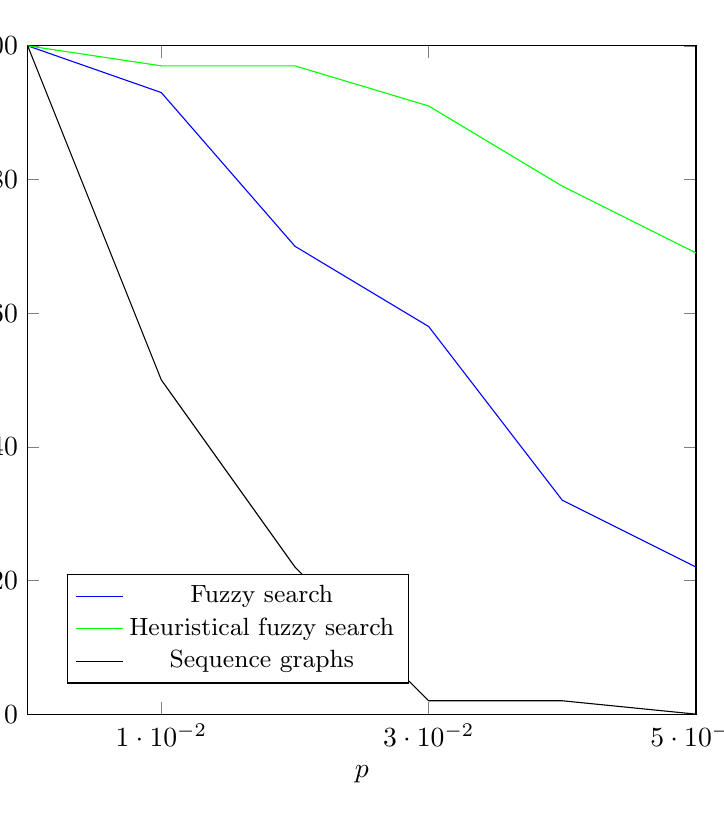
\begin{tikzpicture}[trim axis left,trim axis right]
    \begin{axis}[scale only axis,height=0.7\textwidth,width=0.7\textwidth,xmin=0,ymin=0,xmax=0.05,ymax=100,scaled ticks=false,xtick={0.01,0.03,0.05}, ylabel={Percentage of correctly mapped reads}, xlabel={$p$}, legend style={font=\small, at={(0.57,0.21)}}]
      \addplot[color=blue] coordinates {
        (0, 100-0)
        (0.01,100-7)
        (0.02,100-30)
        (0.03,100-42)
        (0.04,100-68)
        (0.05,100-78)
      };
      \addplot[color=green] coordinates {
        (0, 100)
        (0.01, 97)
        (0.02, 97)
        (0.03, 91)
        (0.04, 79)
        (0.05, 69)
      };
      \addplot[color=black] coordinates {
        (0, 100-0)
        (0.01,100-50)
        (0.02,100-78)
        (0.03,100-98)
        (0.04,100-98)
        (0.05,100-100)
      };
      \addlegendentry{Fuzzy search}
      \addlegendentry{Heuristical fuzzy search}
      \addlegendentry{Sequence graphs}
    \end{axis}
  \end{tikzpicture}
  \caption{Correctly mapped reads from the two tools with $\lambda=2$}
  \label{fig:comparison_correctness}
\end{figure}
\end{document}